\documentclass[]{article}


%-----------------------------------------------------------------------------------------------------------------------------------------
%
%   GLOBALS
%
%-----------------------------------------------------------------------------------------------------------------------------------------
\newcommand{\DOCTITLE}{

}
\newcommand{\DOCAUTHOR}{

}
\newcommand{\DISCLAIMER}
{
    \topskip0pt
    \vspace*{\fill}
    {
    \centering
        \small{
            THIS DOCUMENT IS INTENDED FOR CANADIAN TEAMS ONLY
        }
    }
    \\
    {
    \centering
        \small{
        GO CANADA 
        }
    }
    \vspace*{\fill}
}

\usepackage{lmodern}
\usepackage{amssymb,amsmath}
\usepackage{ifxetex,ifluatex}
\usepackage{fixltx2e} % provides \textsubscript
\ifnum 0\ifxetex 1\fi\ifluatex 1\fi=0 % if pdftex
  \usepackage[T1]{fontenc}
  \usepackage[utf8]{inputenc}
\else % if luatex or xelatex
  \ifxetex
    \usepackage{mathspec}
    \usepackage{xltxtra,xunicode}
  \else
    \usepackage{fontspec}
  \fi
  \defaultfontfeatures{Mapping=tex-text,Scale=MatchLowercase}
  \newcommand{\euro}{€}
\fi
% use upquote if available, for straight quotes in verbatim environments
\IfFileExists{upquote.sty}{\usepackage{upquote}}{}
% use microtype if available
\IfFileExists{microtype.sty}{%
\usepackage{microtype}
\UseMicrotypeSet[protrusion]{basicmath} % disable protrusion for tt fonts
}{}
\ifxetex
  \usepackage[setpagesize=false, % page size defined by xetex
              unicode=false, % unicode breaks when used with xetex
              xetex]{hyperref}
\else
  \usepackage[unicode=true]{hyperref}
\fi
\usepackage[usenames,dvipsnames]{color}
\hypersetup{breaklinks=true,
            bookmarks=true,
            pdfauthor={},
            pdftitle={Canadian Amateur Rocketry Standards and Best Practices},
            colorlinks=true,
            citecolor=blue,
            urlcolor=blue,
            linkcolor=magenta,
            pdfborder={0 0 0}}
\urlstyle{same}  % don't use monospace font for urls
\usepackage{longtable,booktabs}
\usepackage{graphicx,grffile}
\makeatletter
\def\maxwidth{\ifdim\Gin@nat@width>\linewidth\linewidth\else\Gin@nat@width\fi}
\def\maxheight{\ifdim\Gin@nat@height>\textheight\textheight\else\Gin@nat@height\fi}
\makeatother
% Scale images if necessary, so that they will not overflow the page
% margins by default, and it is still possible to overwrite the defaults
% using explicit options in \includegraphics[width, height, ...]{}
\setkeys{Gin}{width=\maxwidth,height=\maxheight,keepaspectratio}
\usepackage[normalem]{ulem}
% avoid problems with \sout in headers with hyperref:
\pdfstringdefDisableCommands{\renewcommand{\sout}{}}
\setlength{\parindent}{0pt}
\setlength{\parskip}{6pt plus 2pt minus 1pt}
\setlength{\emergencystretch}{3em}  % prevent overfull lines
\providecommand{\tightlist}{%
  \setlength{\itemsep}{0pt}\setlength{\parskip}{0pt}}
\setcounter{secnumdepth}{0}

\title{Canadian Amateur Rocketry Standards and Best Practices}
\date{}

% Redefines (sub)paragraphs to behave more like sections
\ifx\paragraph\undefined\else
\let\oldparagraph\paragraph
\renewcommand{\paragraph}[1]{\oldparagraph{#1}\mbox{}}
\fi
\ifx\subparagraph\undefined\else
\let\oldsubparagraph\subparagraph
\renewcommand{\subparagraph}[1]{\oldsubparagraph{#1}\mbox{}}
\fi

%-----------------------------------------------------------------------------------------------------------------------------------------
%
%   PAGE SIZE AND MARGINS
%
%-----------------------------------------------------------------------------------------------------------------------------------------
\usepackage[a4paper,headheight=30pt]{geometry}
%\usepackage[letterpaper, portrait, margin=2in]{geometry}
\addtolength{\topmargin}{-.5in}
\addtolength{\textheight}{1.75in}

\usepackage{graphicx}

\usepackage{fancyhdr}
\pagestyle{fancy}


%-----------------------------------------------------------------------------------------------------------------------------------------
% Page break after sections
%-----------------------------------------------------------------------------------------------------------------------------------------
%\usepackage{titlesec}
%\newcommand{\sectionbreak}{\clearpage}

\lhead{
    %left header content
%    \topskip0pt
%    \vspace*{\fill}
    {
    \centering
        
\includegraphics[height=2.66em]{images/mapleleaf.png}
    }
%    \vspace*{\fill}
}
\chead{
    \topskip0pt
    \vspace*{\fill}
    {
    \centering
        \small{
            THIS DOCUMENT IS INTENDED FOR CANADIAN TEAMS ONLY
        }
    }
    \\
    {
    \centering
        \small{
        GO CANADA 
        }
    }
    \vspace*{\fill}
}
\rhead{
%    \topskip0pt
%    \vspace*{\fill}
    % right header content
    {
    \centering
        
\includegraphics[height=3.0em]{images/mapleleaf.png}
    }
%    \vspace*{\fill}
}
\lfoot{
    % left footer content
    \topskip0pt
    \vspace*{\fill}
    Canada
    Revision 0.0
    \vspace*{\fill}
}
\cfoot{
    % middle footer content
    \topskip0pt
    \vspace*{\fill}
    {
    \centering
    Doc Template \\
    \today
    }
    \vspace*{\fill}
}
\rfoot{
    % right footer content
    \topskip0pt
    \vspace*{\fill}
    \thepage
    \vspace*{\fill}
}
% extend the header into the margins
\usepackage{calc}
\fancyheadoffset[L,R]{\marginparsep+\marginparwidth}

%--------------------------------------------------------------------------------------------------------------
%	My Packages
%--------------------------------------------------------------------------------------------------------------
\usepackage{capt-of}
%--------------------------------------------------------------------------------------------------------------
%	
%	COPY FRONTMATTER AND MAINMATTER AND BACKMATTER COMMANDS
%	
%--------------------------------------------------------------------------------------------------------------
\makeatletter

\newcommand\frontmatter{%
    \cleardoublepage
  %\@mainmatterfalse
  \pagenumbering{roman}}

\newcommand\mainmatter{%
    \cleardoublepage
 % \@mainmattertrue
  \pagenumbering{arabic}}

\newcommand\backmatter{%
  \if@openright
    \cleardoublepage
  \else
    \clearpage
  \fi
 % \@mainmatterfalse
   }

\makeatother

%--------------------------------------------------------------------------------------------------------------
%
%	BEGIN DOCUMENT
%
%--------------------------------------------------------------------------------------------------------------
\begin{document}

%--------------------------------------------------------------------------------------------------------------
%
%	TITLEPAGE
%
%--------------------------------------------------------------------------------------------------------------

%\maketitle

\begin{titlepage}

\newcommand{\HRule}{\rule{\linewidth}{0.5mm}} % Defines a new command for the horizontal lines, change thickness here

\center % Center everything on the page
 
%----------------------------------------------------------------------------------------
%	HEADING SECTIONS
%----------------------------------------------------------------------------------------


\includegraphics[width=200pt]{images/mapleleaf.png}\\[1cm] % Include a logo - this will require the graphicx package
\textsc{\Large Reaction Dynamics Inc.}\\[0.5cm] % Major heading such as course name
\textsc{\large Operations Division}\\[0.5cm] % Minor heading such as course title

%----------------------------------------------------------------------------------------
%	LOGO SECTION
%----------------------------------------------------------------------------------------

\begin{figure}[ht]
    \centering
    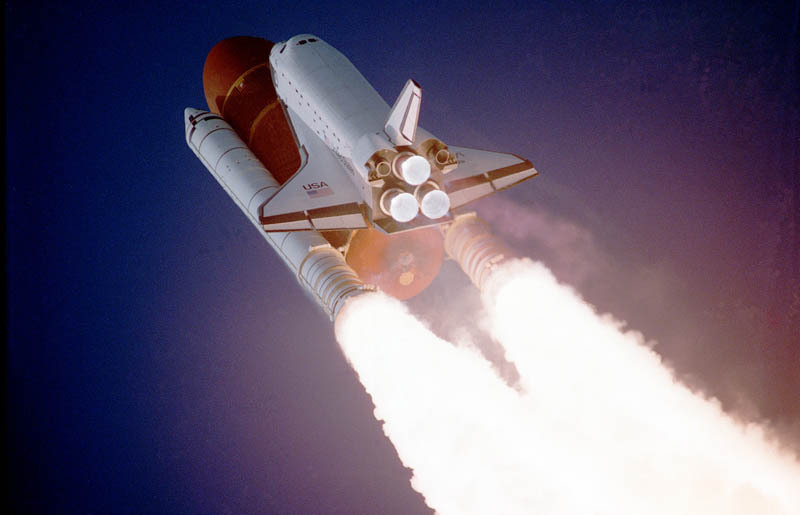
\includegraphics[height=200pt]{images/nasa-rocket-launch-high-quality-24.jpg}\\
\end{figure}

%----------------------------------------------------------------------------------------
%	TITLE SECTION
%----------------------------------------------------------------------------------------

\HRule \\[0.6cm]
{ \Huge \bfseries 
SLV Operations Outline and Field Schedule
}\\[0.4cm] 

\HRule \\[1cm]
 
%----------------------------------------------------------------------------------------
%	AUTHOR SECTION
%----------------------------------------------------------------------------------------
\begin{minipage}{0.4\textwidth}
\begin{flushleft} \large
	\begin{tabular} {r l} 
        \emph{Author(s):} & Someone	\\
	\end{tabular}
\end{flushleft}
\end{minipage}
~
\begin{minipage}{0.4\textwidth}
\begin{flushright} \large
	\begin{tabular} {r l} 
		\emph{Coordinator:} & Someone 		\\
		\emph{Supervisor:}  & Someone 		\\
		\emph{EIR:}         & Someone  		        \\
	\end{tabular}
\end{flushright}
\end{minipage}\\[2cm]

%----------------------------------------------------------------------------------------
%	DATE SECTION
%----------------------------------------------------------------------------------------

{\large \today}\\[2cm] % Date, change the \today to a set date if you want to be precise

\vfill % Fill the rest of the page with whitespace

\end{titlepage}


%--------------------------------------------------------------------------------------------------------------
%
%	FRONT MATTER
%
%--------------------------------------------------------------------------------------------------------------
\frontmatter
\section{Preamble}
The following is a collection of standards and best practices compiled by Canadian rocketry teams based on their experiences with research, design, manufacturing, and testing in a variety of areas. This document is intended as a resource for teams to consult when evaluating their rockets and making design or project decisions, in order to pursue their objectives in the safest and most effective way possible.

This resource is not intended as a binding document on any team. It is understood that every team encounters new and unique problems, both technical and operational, through the course of their work, and the solutions documented here are by no means the best solution for every problem. Teams are encouraged to research and experiment when facing their own challenges, and to contribute to this document if they wish to share any knowledge they have gained through their experience.

This document is organized into a few subheadings now, if you think we need another one just add it. Feel free to add content directly, however, if you see an error or would like to suggest a change use comments or “suggested changes” mode.

\clearpage

{
\hypersetup{linkcolor=black}
\setcounter{tocdepth}{3}
\tableofcontents
\clearpage
}

\listoftables
\listoffigures
\clearpage


%--------------------------------------------------------------------------------------------------------------
%
%	MAIN MATTER
%
%--------------------------------------------------------------------------------------------------------------
\mainmatter

%--------------------------------------------------------------------------------------------------------------
% body
%--------------------------------------------------------------------------------------------------------------
\subsection{List of Abbreviations}\label{list-of-abbreviations}
\begin{longtable}[c]{@{}llll@{}}
\toprule
Abbreviation & Description & Function of & Units\tabularnewline
\midrule
\endhead
AOA, \(\alpha\) & Angle of Attack & & radians\tabularnewline
COP & Center of pressure & & N/A\tabularnewline
COG & Center of gravity & time & N/A\tabularnewline
Re & Reynolds Number & \( \rho,\mu,\vec{v},L \) &
dimensionless\tabularnewline
\(Re_{crit}\) & Critical Reynolds Number & \( \rho,\mu,\vec{v},L \) &
dimensionless\tabularnewline
\(I_{zz}\) & Pitch/Yaw Moment of Inertia & time & \(m^4\)\tabularnewline
D & Drag Force (combined) & & N\tabularnewline
W & Weight of the Rocket & & N\tabularnewline
R & Specific Gas Constant & & \(J kg^{-1} K^{-1}\)\tabularnewline
T & Thrust of the Rocket & & N\tabularnewline
\(t_f\) & Fin thickness & distance & m\tabularnewline
\(L_{cf}\) & Aerodynamic Chord Length of Fins & distance &
m\tabularnewline
c & Speed of sound & \( \sqrt{\gamma RT} \) &\tabularnewline
\(R_a\) & Surface Finish & \( distance \) & microns\tabularnewline
M & Mach Number & \( \vec{v}, c \) & dimensionless\tabularnewline
\(D_{pa}, C_{pa}\) & Parasitic Drag Force, Coefficient &
&\tabularnewline
\(D_{fb}, C_{fb}\) & Body Drag Force, Coefficient & &\tabularnewline
\(D_{fp}, C_{fp}\) & Fin Pressure Drag Force, Coefficient &
&\tabularnewline
\(D_{pr}, C_{pr}\) & Pressure Drag Force, Coefficient & &\tabularnewline
\(D_{in}, C_{in}\) & Interference Drag Force, Coefficient &
&\tabularnewline
\(D_{ba}, C_{ba}\) & Base Drag Force, Coefficient & &\tabularnewline
\(D_{sk}, C_{sk}\) & Skin Friction Drag Force, Coefficient &
&\tabularnewline
\(D_{aoa}, C_{aoa}\) & Additional Angle of Attack Drag Force,
Coefficient & &\tabularnewline
\(C_{MC}\) & Corrective Moment Coefficient & &\tabularnewline
\(C_{FN}\) & Normal Force Coefficient & &\tabularnewline
\(C_{PDM}\) & Propulsive Damping Moment Coefficient & &\tabularnewline
\(C_{ADM}\) & Aerodynamic Damping Moment Coefficient & &\tabularnewline
\(A_{wb}\) & Area of Wetted Body & & \(m^2\)\tabularnewline
\(A_{wf}\) & Area of Wetted Fins & & \(m^2\)\tabularnewline
\(A_{fr}\) & Frontal Reference Area & & \(m^2\)\tabularnewline
\(A_{fp}\) & Fin Planform Area & & \(m^2\)\tabularnewline
\(A_{fe}\) & Exposed Fin Planform Area & & \(m^2\)\tabularnewline
OD,\(\phi_{bt}\) & Outer Diameter & & m\tabularnewline
L & Total Length of Rocket & & m\tabularnewline
h\_n & Height of the nose cone & & m\tabularnewline
\(S_{fc}\) & Thrust Specific Fuel Consumption & &
\(\dfrac{g}{s}\cdot \dfrac{1}{N} = \dfrac{s}{m}\)\tabularnewline
\(\dot{m}_{fc}\) & Mass Flow Rate due to Fuel Consumption & &
\(\dfrac{g}{s}\cdot \dfrac{1}{N} = \dfrac{s}{m}\)\tabularnewline
\(T_{avg}\) & Average Thrust & & N\tabularnewline
\(t_{burn}\) & Burn Time & & s\tabularnewline
\(m_{m_t}\) & Total Motor Mass & & g\tabularnewline
\(W_{m_t}\) & Total Motor Weight & & N\tabularnewline
\(F_N\) & Aerodynamic Normal Force & & N\tabularnewline
\(F_A\) & Aerodynamic Axial Force & & N\tabularnewline
\(F_L\) & Aerodynamic Lift Force & & N\tabularnewline
\(S_{lm}\) & Longitudinal Stability Margin & & Calibers\tabularnewline
\(f_B\) & Fineness Ratio & & dimensionless\tabularnewline
\(\mu\) & Dynamic Viscosity & & \(N s / m^2\)\tabularnewline
\(\nu\) & Kinematic Viscosity & \(\mu\), \(\rho\) &
\(m^2/s\)\tabularnewline
\(\lambda\) & Angular Acceleration & & \(rad/s^2\)\tabularnewline
\(\omega\) & Angular Velocity & & \(rad/s\)\tabularnewline
\(\theta\) & Angular Position & & \(radians\)\tabularnewline
\bottomrule
\end{longtable}

\captionof{table}{List of Abbreviations}
\clearpage

%\section{Section 0 - Explanation of the Standards}\label{section-0}
%	% section 1

\subsection{Section 1}\label{section1}

some text goes here


%	\clearpage


\section{Section 1 - Flight Dynamics, Prediction and Simulation}\label{section-1}
	\begin{itemize}
\item IREC requires that your static margin off the rail is at least 1.0
\item However, if your predictions/simulations only give you a stability factor of 1, bear in mind that your actual flight may show a lower thrust than expected from testing.
\item This may adversely impact your speed off the rail, and drop your margin below 1. Be aware, and plan for that.
\end{itemize}

	\clearpage
	
\section{Section 2 - Aerostructures}\label{section-2}
	\subsection{General Safety Guidelines}
\begin{itemize}
\item If you have any pressure vessels in your rocket (combustion chamber, oxidizer or fuel tank, whatever), hydrostatic test it to a decent factor of safety.
\item In this instance, please don't let "decent" be anything less than 1.5. Even that's probably pushing it.
\item Inspect EVERYTHING once you get to SAC. It’s possible that some gear, including flight components were damaged during their travels from Canada to competition. Don’t fly damaged hardware, as your successful hydrostatic tests no longer apply.
\item Writing an inspection checklist will greatly streamline the process of checking all flight hardware, so doing so is highly recommended.
\end{itemize}

\subsection{Structural Vibrations}
\subsubsection{Analyzing Fins for aeroelastic loads}

NACA TN-4197 presents a simplified criterion for determining the air speed at which rocket fins will experience destructive fin flutter with the following equation:
\begin{equation}
V_f = a\sqrt{\frac{G_E}{\frac{39.3A^3}{(\frac{t}{c})^3(A+2)}(\frac{\lambda+1}{2})(\frac{P}{P_0})}}
\end{equation}

Where $V_f$ is the flutter speed, $a$ is the speed of sound, $G_E$ is the shear modulus, $A$ is the aspect ration, $\lambda$ is the taper ratio, $P$ is the pressure at the vehicle’s current altitude, $P_0$ is the standard pressure at sea level (considered to be 1 bar), $t$ is the thickness of the fin and $c$ is the root chord of the fin.
	The units presented by NACA to be used in these calculations are imperial. However, in a few cases, units of one’s choice may be used, such as with the ratio of sea-level pressure to current pressure, the ratio of thickness to root chord, or for the velocities. In these cases, as long as both terms in the ratio have the same unit, the final result will be correct (i.e., if the speed of sound is in meters per second, the final result will be in meters per second). The critical exception is that the shear modulus must be in pounds per square inch.

	\clearpage
	
\section{Section 3 - Recovery Systems}\label{section-3}
	\subsection{General Safety Guidelines}
\begin{itemize}
\item This system stops your rocket from falling on human beings at terminal velocity. If there is anything more than an infinitesimal chance that it will fail, then you are recklessly endangering human lives. This system is by far the most safety critical.
\item Test it. Make sure it doesn't just work, make sure it works flawlessly. If it doesn't work flawlessly under laboratory conditions, It’s possible that it will function even worse in the field.
\item This goes without saying for all points in this document, but bears explicit statement here: IREC publishes their own set of standards for operation and testing of many flight components. While these (the Canadian Rocketry) guidelines are not binding, theirs (IREC’s) are, and thus must be met or exceeded (go for exceeded. Many of their standards are bare minimum, and you can probably do better)
\end{itemize}

\subsection{Ground Testing of Recovery Systems}
The way to properly validate the system by which a parachute is ejected from a rocket is the recovery ground test. The following is a generalized guideline for performing a recovery ground tests safely and assessing the results to determine if your system is functional.
\par
The minimum safety equipment requirements for any personnel directly involved in testing are listed below. Personnel directly involved in the test are defined as personnel who are responsible for handling the packing of any pyrotechnic charges, or being within 30 feet of the rocket when it is loaded with any pyrotechnic substances or has any stored-energy.
\begin{itemize}
\item Safety Glasses
\item Face Shields (if it is expected that the test may produce debris)
\item Flame-resistant gloves (if parts are expected to be hot after the test)
\item Closed Toe Shoes
\item Long pants and Long Sleeved Shirt (if it is expected that the test may produce debris)
\end{itemize}

The following requirements for the test site should be observed:
\begin{itemize}
\item The rocket must be placed on a stand of some kind and should be kept horizontal. A hanging cradle for the rocket is also acceptable, but both halves of the rocket must be attached to the cradle and must not become detached from the cradle during the test.
\item It is advisable that any solid part being ejected be covered in EVA foam or the ground where it will land be covered in foam (for the protection of the part)
\item The area 30 feet in front and behind the rocket should be cleared of people.
\item Non-essential people should not be in the area where parts will be ejected and should preferably be 15 feet away.
\item The area should be cleared of any flammable material if pyrotechnics are being used for ejection
\item There must be no ignition sources in the area if pyrotechnics are being used for ejection (that means no smoking)
\item A fire-extinguisher must be kept on hand if pyrotechnics are being used for ejection
\end{itemize}

	\clearpage
	
\section{Section 4 - Payloads}\label{section-4}
	\subsection{General Safety Guidelines}
\begin{itemize}
\item If your payload contains electrical components, make sure your payload wiring doesn't come close to your avionics/recovery wiring. If the wiring does does, then it should also be meet or exceed the Safety Critical wiring standard that IREC publishes. You can find that standard here \url{http://www.soundingrocket.org/uploads/9/0/6/4/9064598/wiring_guidelines_v3.pdf}
\item If you have a deployable payload, its recovery system should be subject to the same level of testing that your main rocketry recovery system is. Redundant electrics, flawless tests, etc. 
\end{itemize}

	\clearpage
	
\section{Section 5 - Avionics and Groundstations}\label{section-5}
	\subsection{General Safety Guidelines for Recovery Deploying Flight Electronics}
\begin{itemize}
\item Please have redundant electronics. You should have 2 completely separate circuits. Redundant altimeters, pyro-cutters, wiring, power sources, everything. If you don't have dual redundancy, you're begging Murphy’s law to ruin your day.
\item Use a commercial altimeter
\end{itemize}

\subsection{General Safety Guidelines for designing a launch control ground station}
\begin{itemize}
\item Your ground station should probably have a key switch (or some other way of disabling it while personnel are at the launch pad), and the key should be with launch pad personnel while they are at the pad.
\item If your client-side (or control side, human side, base camp side, whatever) ground station loses contact with your tower-side (or rocket side, or whatever), the tower-side ground station should be programmed to keep itself in the safest possible state (don't turn on ignition, stop filling the rocket with fuel, etc).
\item Your ground station needs to work from outside the Minimum Safe Distance set by ESRA. In 2017, this was 2000 feet, but launch control was located 3000' away. So aim for 3000. And give yourself some breathing room. About a mile should be fine.
\item If you're implementing your own communications protocol (probably overkill, but some projects do), then you need checksums and acknowledgments baked into that protocol. It should not be conceptually possible for your tower side station to do anything that the client side station did not ask it to do. It should also be impossible to hit any kind of deadlock or out of phase-ness.
\item If you're writing code (for ground station specifically, but this really goes for any safety critical software), write it in pseudo-code first, then get it reviewed by at least 2 people who know what they're doing, then write it, then unit test it to the best of your ability. This code is responsible for keeping people alive. Having it in pseudo-code makes it easier to understand for new people, and makes it easier to debug in case of strange behaviour.
\end{itemize}

	\clearpage
	
\section{Section 6 - Propulsion}\label{section-6}
	\subsection{General Safety Guidelines}
\begin{itemize}
\item This will vary wildly based on your propulsion mechanism. I’m not an expert in this area, but the only advice that I feel qualified to give is that if you are building your own engine, please conduct at least 2 static test fires of it if possible, as close to launch condition as is possible. 
\item During static fires, maintain the same level of care as you would when performing a full flight. Draft procedures and checklists, and follow them as if you were at competition. These tests can be more than just validation for your engine, they can also validate your operations checklists, which is also extremely valuable.
\end{itemize}

	\clearpage
	
\section{Section 7 - Competition and Field Operations}\label{section-7}
	\subsection{Why you need more checklists}
    \begin{itemize}
        \item Once you hit the desert, assume that everyone loses the ability to think. It's 40 degrees, everyone has heatstroke, and they're probably operating at about the same level as your standard alcoholic. It's much harder to make dangerous mistakes when following a checklist.
    \end{itemize}

\subsection{How to do a great checklist}
    \begin{itemize}
        \item Know your failure modes, know at what point they could arise during your checklist, and write down the appropriate abort procedure to take to minimize risk at that failure mode.
        \item No step in your procedure is optional. If it’s written down, it’s mandatory. If it’s not mandatory, it’s unnecessary and should be removed.
        \item Have procedures for every off-nominal scenario, regardless of how unlikely it is. You should do this for two reasons: 
        \begin{enumerate}
            \item There is always a possibility that you’ll end up in that scenario anyways, and you want to be prepared rather than scrambling to figure out what you should do next.
            \item Creating and reviewing off-nominal procedures forces you to become more familiar with the procedure as a whole, and lets you identify anything that you may have overlooked or any mistakes you might have made.
        \end{enumerate}
        \item Once you have a complete checklist, read it out with all people who are going to be involved in it. If you notice anything wrong or potentially unsafe in your checklist, change it. Then read it out with all your people again. Spending an extra few hours working at home is worth it if it makes desert operations run smoother and safer.
        \item If your primary plan puts human being inside the Minimum Safe Distance (2000 feet) while your rocket is in an unsafe state (solid engine: ignition leads are hooked up, hybrid engine: Ignition leads are hooked up or your rocket has any amount of pressurized fluid in it), then you have fucked up. Rewrite it. If you have to make changes to other parts of your system, then do so. Rockets are dangerous, and the best way of minimizing their risk is staying away from them while they are in a dangerous state.
    \end{itemize}

\subsection{Launch Operations}
    This section mostly applies to hybrid rockets, which require additional steps due to filling procedures.
    \begin{itemize}
        \item Have defined roles for everyone who will be part of operations procedures. Before you even get to the desert, you need to know exactly how many launch technicians will be necessary, who those technicians are going to be, and what each technician is going to do.
        \item Your operations procedure must unambiguously describe every action that will be performed by every technician, and identify who (by role) will be performing it. You don’t want to start filling your rocket and then realize that you don’t have enough people to finish the process.
        \item Every technician involved in launch operations should be familiar with every step that they need to perform - both nominal and off-nominal. Do at least one read-through of the procedure with everyone involved, and at least one dry run or simulated launch that gets as close to actual procedures as possible without placing the rocket in an unsafe state. Make any changes that are necessary, and practice any parts that get changed until everything runs perfectly. You want to eliminate any potential issues now, rather than trying to improvise while your rocket is filling with oxidizer.
        \item Exactly one person should be given control of operations during launch procedures, and identified as such (Flight Director, Technician In Control, etc.). This person’s only role should be to read out each step of the operations procedure to the technicians responsible for performing it, and to proceed to an off-nominal or abort procedure if necessary. Your flight director should be familiar with every single step of the procedure, and should have a physical copy in front of them during fill and launch operations.
        \begin{itemize}
            \item I can’t stress enough that the flight director should only be responsible for coordinating the procedure and directing the technicians. Hybrid launch operations are complicated and time-sensitive, and if you accidentally miss a single step, you could easily both jeopardize your chances of a nominal flight and put lives in danger. The flight director needs to be able to concentrate fully on the procedure. That means that you should have a separate technician (or technicians) operating any ground stations, including ignition.
        \end{itemize}
        \item If, at any point during your launch procedure, you have personnel in multiple locations, the flight director must have radio communication with them. If communication is lost, you need to stop operations immediately. You don’t want to be sending an ignition signal when your technicians are at the pad standing 20 feet from the rocket.
        \item Perform all relevant checks before you start launch operations, rather than during. Have a checklist of checks to perform before starting the procedure. This should include things like:
        \begin{itemize}
            \item Ensure your technicians have radios 
            \item Electrical checks on ground stations and launch systems
            \item Make sure the range is clear
        \end{itemize}
        \item During launch operations, the flight director should give instructions by first identifying the technician who will perform the action and then by stating the instruction (turn this valve, make this electrical connection, press this button, etc.). The flight director should wait for confirmation that the action has been successfully performed before continuing. Launch ops are stressful and can be hectic. You don’t want things to go wrong because one of your technicians misheard you or couldn’t keep up with the pace you were reading.
    \end{itemize}

\subsection{How to survive in the desert}
    Each person should have all the items listed below. The items should be checked by a team safety officer or supervisor prior to going in-field
    \begin{enumerate}
    \item A wide-brim hat or baseball cap with a covering for the back of the neck
    \item Sunscreen, 70 spf or higher (each individual must have a bottle)
    \item Water, at least 5 liters each (or a sports drink like Powerade)
    \item Team shirt
    \item Long pants (light cotton suggested)
    \item Closed toe shoes with socks
    \item Safety glasses (preferably tinted)
    \item Bandanas or something to cover the face
    \end{enumerate}

    The following equipment should be brought to the desert and only one item is necessary for the entire team. The responsibility for making sure this equipment should fall on the team captain or relevant safety officer
    \begin{enumerate}
        \item Properly sized tent
        \item A number of chairs equivalent to the number of team members in the desert
        \item At least 2 tables
        \item Additional water, at least 3 cases of 24 water bottles. A sports drink like Powerade can also be used
        \item Additional sunscreen
        \item Food
        \item Cars with sufficient space to carry all team members to a from the launch site. These vehicles should have air conditioning, they should not be convertibles and they should not be too low to the ground
        \item A large first aid kit
        \item Face Shields
        \item Salt
    \end{enumerate}

    The following outlines some of the greatest hazards presented by the desert environment. Remember, never, ever be alone in the desert. Make sure you are always with someone.
    \begin{enumerate}
        \item Blowing dust: High winds are often present in the desert. These high winds can create a significant amount of blowing dust or sand. If these conditions are encountered, the safety goggles and bandanas should be used to protect the face
        \item Strong Sunlight: Always use sunscreen and a wide-brim hat
        \item Extreme heat and dryness: The temperature can rise up to 45 degrees Celsius with virtually no humidity. In these conditions, heat stroke and dehydration are real and present dangers. Light clothing must be worn, so as to avoid overheating. As well, copious amounts of water must be consumed. If you are not urinating, then you are not drinking enough water. Finally, constant perspiration can deplete the amount of salt present in the body. Thus, a large amount of salt must be consumed or sports drinks must be consumed along with water. If you begin to feel dizzy or lightheaded, sit down in the shade and drink large quantities of water.
        \item Poisonous Animals: The desert is home to animals such as scorpions, tarantulas, and rattlesnakes. Avoid these at all costs. Take extra care when climbing through jumbled rocks. Avoid turning over rocks unless it is with a long stick. If bitten by one of these creatures, report to paramedics or emergency services immediately. If you cannot positively identify the creature, take a picture of it so it can be more easily recognized by medical personnel who can then administer the appropriate antivenin. If Killer Bees are encountered, run away as fast as possible.
        \item Cacti: The desert has many forms of cacti, all of which have spines and needles which could cause significant discomfort. Wear long pants and high boots to avoid having needles impaled into your legs. If you do end up with cactus spines embedded in you skin, remove with pliers and treat the wound like any other cut.
        \item Additional Competition Safety to be observed at the launch site:
        \begin{enumerate}
            \item Driving: Do not drive or stay in a car while there is a rocket about to be launched or in the air. Range safety officers will keep you informed as to the current safety condition of the camp.
            \item Rocket Emergencies: If you hear the call “Heads-up!” or hear an air raid siren, then this means that there is a critical safety hazard which has been caused by a flying rocket. Either it has gone ballistic or has broken apart causing a significant amount of debris. Immediately exit from any form of shelter and watch the sky. Listen for any calls from range safety officers.
            \item Work Areas: Do not enter any work areas without proper safety equipment and authorization. Do not enter a work area that does not belong to your team unless invited to do so.
            \item Desert Recovery: When venturing into the desert to recover a rocket, remember to bring adequate water and gear. Do not venture into the desert without a certified BARQ radio operator. The radio operator is necessary as he carries a GPS as has constant contact with basecamp. Thus, he can easily guide the team back to base and stay aware of any hazards announced by Range Safety Officers. Make sure all personnel venturing into the desert are of adequate physical fitness to make the trip.
            \item Additional Safety Hazards: If you see another team failing to follow proper safety guidelines (such as improper protection when working with black powder) inform them of their error. If they do not correct it, inform a Range Safety Officer.
        \end{enumerate}
    \end{enumerate}

	\clearpage
	
\section{Section 8 - General Testing Guidelines}\label{section-8}
	\begin{itemize}
\item Test often, test to failure.
\item Your tests should demonstrate that you know the failure modes, and they should demonstrate that the failure mode is safe
\end{itemize}

	\clearpage
	
\section{Section 9 - Documentation}\label{section-8}
	\begin{itemize}
\item Documentation exists for 2 reasons:
\begin{enumerate}
\item Help people use your system. So write a user's guide, make it simple enough that people who have never seen a rocket before can operate your system
\item Help people fix your system when it invariably breaks (Murphy's law applies doubly in rocket science). You, as the designer, are responsible for knowing how your system can fail, how to diagnose every failure mode, and how to fix it. Assume that the person who needs to fix your gear has never met you before. They should still be able to fix it.
\end{enumerate}
\end{itemize}

	\clearpage

%--------------------------------------------------------------------------------------------------------------
%
%	BACK MATTER
%
%--------------------------------------------------------------------------------------------------------------
%\backmatter

%--------------------------------------------------------------------------------------------------------------
%--------------------------------------------------------------------------------------------------------------
\mainmatter
\end{document}
